%---------change this every homework
\def\yourid{mst3k}  % substitute your userED
\def\collabs{collaborators} % substitute your collaborators
\def\sources{sources} % substitute your sources
% -----------------------------------------------------
\def\duedate{September 24, 2025 at 11:59p}
\def\pnumber{3}
%-------------------------------------

\documentclass[10pt]{article}
%\documentclass[tikz,border=10pt]{standalone}
\usepackage{dsa2}
\usepackage{float}
\usepackage{tikz}
\usepackage{listings}


\begin{document}
\thispagestyle{empty}
\handout


%%%%%%%%%%%%%%%%%%%%%%%%%%%%%%%%%%%%%%%%%%%%%%%%%%%%%%%%
\begin{problem} Graph Cycles \end{problem}

Consider the problem of needing to remove cycles from a graph.

\begin{enumerate}
    \item Explain how you would remove all cycles from a graph using only DFS. You should describe your algorithm so that it removes the minimum number of edges in order to make it an acyclic graph (i.e., you cannot just say "remove all edges from the graph").

      \solution{
        % Put your solution here.
      }

    \item What is the running time of that algorithm?  Explain why.

      \solution{
        % Put your solution here.
      }

\end{enumerate}

%%%%%%%%%%%%%%%%%%%%%%%%%%%%%%%%%%%%%%%%%%%%%%%%%%%%%%%%

\begin{problem} Minimum Spanning Tree \end{problem}

Find the minimum spanning tree of the following graph.  Each edge in the graph below is labelled with a letter and its weight.  If you encounter a situation where there are two edges of the same weight to consider, then consider the one earlier alphabetically.  The answer should be a space separated list of node letters, in alphabetical order, such as: {\tt A B C D E F}.  Also provide the cost of that tree.



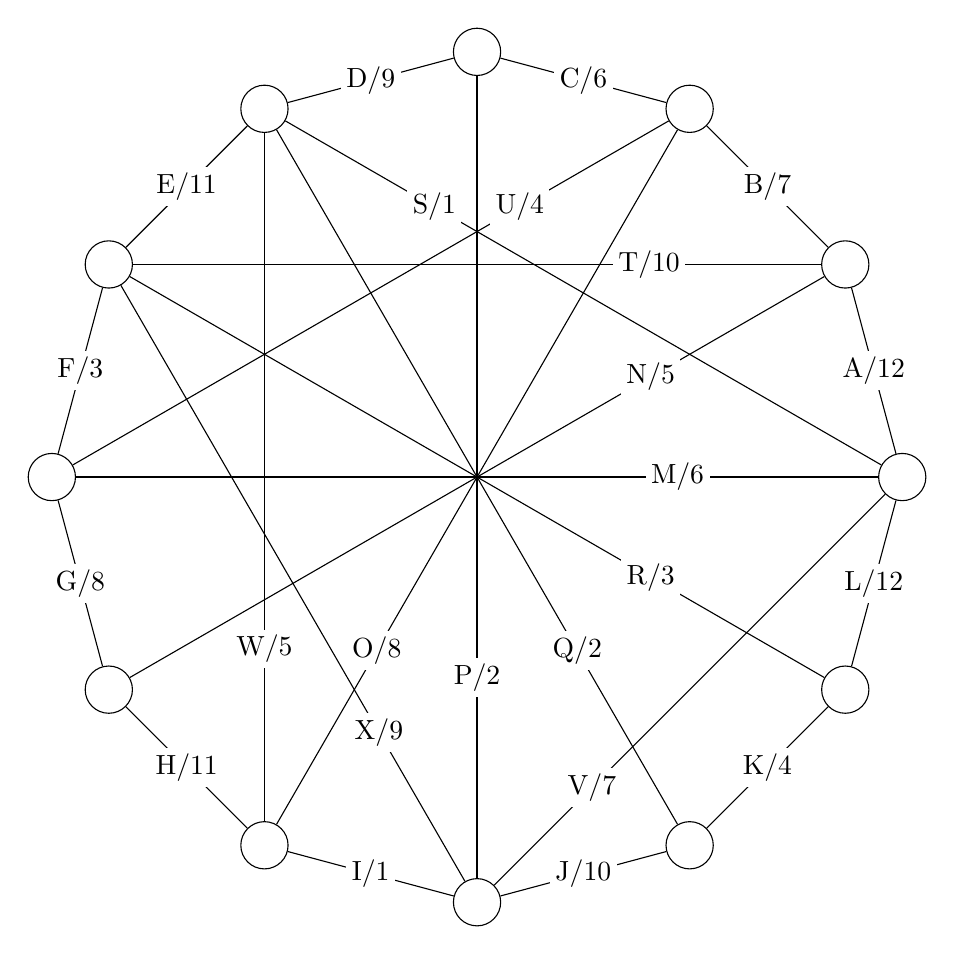
\begin{tikzpicture}[scale=3,
  every node/.style={circle,draw,minimum size=6mm,inner sep=0pt},
  every edge quotes/.style={fill=white,font=\small,inner sep=1pt}
]

% place 12 nodes on a circle (no text inside)
\foreach \i in {1,...,12}{
  \node (N\i) at ({360/12 * (\i-1)}:1.8) {};
}

% edges: 12-ring + 12 chords with letters and weights
\path[every node/.style={->,
    fill=white,inner sep=2pt}]
 (N1) edge [] node [] {A/12} (N2)
 (N2) edge [] node [] {B/7} (N3)
 (N3) edge [] node [] {C/6} (N4)
 (N4) edge [] node [] {D/9} (N5)
 (N5) edge [] node [] {E/11} (N6)
 (N6) edge [] node [] {F/3} (N7)
 (N7) edge [] node [] {G/8} (N8)
 (N8) edge [] node [] {H/11} (N9)
 (N9) edge [] node [] {I/1} (N10)
 (N10) edge [] node [] {J/10} (N11)
 (N11) edge [] node [] {K/4} (N12)
 (N12) edge [] node [] {L/12} (N1)
 % chords
 (N1) edge [] node [near start] {M/6} (N7)
 (N2) edge [] node [near start] {N/5} (N8)
 (N3) edge [] node [near end] {O/8} (N9)
 (N4) edge [] node [near end] {P/2} (N10)
 (N5) edge [] node [near end] {Q/2} (N11)
 (N6) edge [] node [near end] {R/3} (N12)
 (N1) edge [] node [near end] {S/1} (N5)
 (N2) edge [] node [near start] {T/10} (N6)
 (N3) edge [] node [near start] {U/4} (N7)
 (N1) edge [] node [near end] {V/7} (N10)
 (N5) edge [] node [near end] {W/5} (N9)
 (N6) edge [] node [near end] {X/9} (N10);

\end{tikzpicture}

\solution{
  % Put your solution here.
 }


%%%%%%%%%%%%%%%%%%%%%%%%%%%%%%%%%%%%%%%%%%%%%%%%%%%%%%%%

\begin{problem} Square Root \end{problem}

You are to design a {\em divide-and-conquer} algorithm for finding the square root of a positive integer.  If the square root is an integer, it should return that.  Otherwise, if it is between $x$ and $x+1$, it should return $x$.  It should run in $\Theta(\log n)$ time.  {\em Hint: think of a binary search.}


\begin{enumerate}
    \item Write the algorithm in pseudo-code.  This pseudo-code should be in Python-like or Java-like syntax.  This -like part means that we are not going to check for exact Python or Java syntax, but look at it as pseudo-code.  But the formatting, indentation, etc., should be like Python (or Java).  We recommend using the {\tt lstlisting} environment for your pseudo-code.  You can see how that environment works at \url{https://www.overleaf.com/learn/latex/Code_listing}.  {\bf NOTE:} your {\tt lstlisting} environment has to be outside your {\tt solution} environment.

\solution{}\begin{lstlisting}
  % Put your solution here.
\end{lstlisting}

    
    \item What is the recurrence relation for that algorithm?  (You do not need to determine its running time)
    
    \solution{
      % Put your solution here.
    }

\end{enumerate}


%%%%%%%%%%%%%%%%%%%%%%%%%%%%%%%%%%%%%%%%%%%%%%%%%%%%%%%%

\begin{problem} Finishing up Maximum Array Subsequence \end{problem}

Write the algorithm for the {\tt dividingLineSolution(A,first,last)} function discussed in class, which is used in the Maximum Subarray Sum algorithm (the first slide set on divide and conquer).  It is an iterative function.  Like the above, we recommend the {\tt lstlisting} environment.  Again, either Python-like or Java-like syntax.

\solution{}\begin{lstlisting}
  % Put your solution here.
\end{lstlisting}



%%%%%%%%%%%%%%%%%%%%%%%%%%%%%%%%%%%%%%%%%%%%%%%%%%%%%%%%

\end{document}
